\documentclass{standalone}
\usepackage{castle_of_magic}
\usetikzlibrary{backgrounds}
\usepackage{contour}
\contourlength{0.66pt}
\usepackage{fontspec}
\setmainfont[Scale=3.0]{Tex Gyre Chorus}

\definecolor{lightbluestone}{HTML}{f3f7fd}


\begin{document}
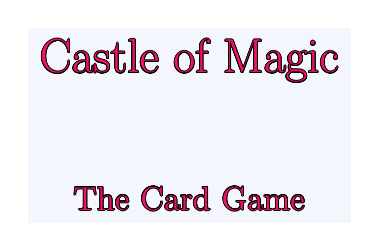
\begin{tikzpicture}[background rectangle/.style={fill=lightbluestone}, show background rectangle]
%\clip (-5.49,-4.3) -- (-5.49, 4.3) -- (5.69,4.3) -- (5.69,-4.3) -- cycle;
%\node at (0,0) {\includegraphics[scale=0.1]{Images/blue_stone_wall_vector.png}};
\node[inner sep=0pt] at (0,2.75) {\contour{black}{\textcolor{WildStrawberry}{\LARGE Castle of Magic}}};
\node[inner sep=0pt] at (0,1.0) {\contour{black}{\textcolor{WildStrawberry}{\large The Card Game}}};
\end{tikzpicture}
\end{document}